%\documentclass[tikz,border=3mm]{standalone}
\documentclass[tikz]{standalone}
\begin{document}
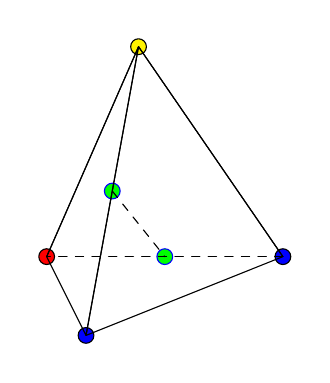
\begin{tikzpicture}[line join = round, line cap = round]
    \pgfmathsetmacro{\factor}{sqrt(3)};
    \coordinate [label=above:] (A) at (0,3,0);
    \coordinate [label=right:] (B) at (1.5,0,-\factor/2);
    \coordinate [label=below:] (C) at (0, 0, \factor);
    \coordinate [label=left:] (D) at (-1.5,0,-\factor/2);

    \coordinate (M1) at (0,1.5,\factor/2);
    \coordinate (M2) at (0,0,-\factor/2);

    %\draw[->] (0,0) -- (3,0,0) node[right] {$x$};
    %\draw[->] (0,0) -- (0,4,0) node[above] {$y$};
    %\draw[->] (0,0) -- (0,0,3) node[below left] {$z$};
    %\foreach \i in {A,B,C,D}
    %    \draw[dashed] (0,0)--(\i);
    %\draw[-, fill=red!30, opacity=.5] (A)--(D)--(B)--cycle;
    %\draw[-, fill=green!30, opacity=.5] (A) --(D)--(C)--cycle;
    %\draw[-, fill=purple!30, opacity=.5] (B)--(D)--(C)--cycle;
    \draw[fill=yellow] (0, 3, 0) circle (0.1);
    \draw[fill=blue] (1.5,0,-\factor/2) circle (0.1);
    \draw[fill=blue] (0, 0, \factor) circle (0.1);
    \draw[fill=red] (-1.5,0,-\factor/2) circle (0.1);

    \draw[blue, fill=green] (0,1.5,\factor/2) circle (0.1);
    \draw[blue, fill=green] (0,0,-\factor/2) circle (0.1);

    \draw[dashed] (M1)--(M2);

    %\draw[dashed, color=gray] (A) to [bend left] (C);

    \draw[-] (D)--(A)--(B);
    \draw[dashed] (B)--(D);
    \draw[-] (A)--(D)--(C)--cycle;
    \draw[-] (A)--(B)--(C)--cycle;
\end{tikzpicture}
\end{document}